\subsection{Implementação computacional}
\label{subsec:implementacao}

\subsubsection{Simulação em Simulink}

\begin{figure}[htbp]
\centering
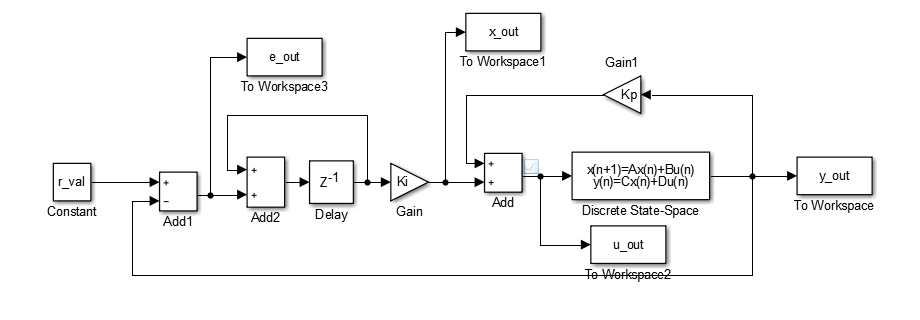
\includegraphics[width=.88\textwidth]{malha_de_controle.png}
\caption{Malha de controle montada em Simulink.}
\label{fig:malha_de_controle_simulink}
\end{figure}

Depois de determinar os ganhos do controlador PI, eles foram testados com o objetivo de avaliar o comportamento da malha diante das incertezas paramétricas consideradas. 

Como pode ser visto na Figura \ref{fig:malha_de_controle_simulink} a implementação do modelo no Simulink foi realizada utilizando um bloco \textit{Discrete State-Space} para representar a dinâmica da planta, uns blocos \textit{Gain} para aplicar os ganhos proporcional e integral, um bloco \textit{Delay} para realizar a ação integral, e um bloco \textit{Constant} para aplicar a referência.

Para avaliar o comportamento da malha fechada em diferentes condições de operação, desenvolveu-se um script de Matlab que executa o modelo de Simulink para as oito combinações extremas dos parâmetros incertos $\gamma_{ob}$, $\mu_m$ e $\mu_o$. Em cada execução, as matrizes da planta são atualizadas no \textit{workspace} global do MATLAB, graças ao bloco \textit{To Workspace}. As condições numéricas e as respostas obtidas são apresentadas na Subseção~\ref{subsec:resultados_simulink}.

\newpage
\subsubsection{Arquitetura da plataforma embarcada}

Depois da simulação em Simulink, a malha de controle foi reproduzida em uma plataforma embarcada \cite{maradiaga2026repositorio}, composta por dois microcontroladores ESP32, programados em linguagem C por meio da \textit{framework} ESP-IDF. Nesta emulação, a lei de controle e a planta foram executados em unidades computacionais distintas, conectadas por meio de uma interface UART.

A arquitetura adotada é apresentada na Figura~\ref{fig:arquitetura_embarcada}. A cada tick de relógio, o ESP32 controlador calcula a ação de controle $u(k)$ e a encaminha ao ESP32 planta através de um pacote UART. A planta recebe o pacote, processa os dados, atualiza seu estado interno e envia a saída $y(k)$ ao controlador por meio de um outro pacote, fechando a malha de realimentação.

\begin{figure}[htbp]
\centering
\begin{tikzpicture}[
 font=\small, >=Latex,
 unit/.style={draw=navyblue,fill=lightblue,rounded corners=3pt,align=center,minimum width=4.0cm,minimum height=1.45cm,line width=.75pt},
 pc/.style={draw=black!70,fill=warmgray,rounded corners=3pt,align=center,minimum width=6.5cm,minimum height=1.55cm,line width=.75pt},
 smallunit/.style={draw=black!65,fill=white,rounded corners=2pt,align=center,minimum width=3.4cm,minimum height=.9cm},
 link/.style={-{Latex[length=2.2mm]},thick},
 wireless/.style={{Latex[length=2.2mm]}-{Latex[length=2.2mm]},densely dashed,thick,navyblue}
]
\node[unit] (ctrl) at (-4,2.35) {\textbf{ESP32 -- Controlador}\\ Implementa o PI discreto\\\footnotesize $f=100\,\mathrm{Hz}$};
\node[unit] (plant) at (4,2.35) {\textbf{ESP32 -- Planta}\\ Emula o modelo farmacocinético\\\footnotesize Atualização a cada pacote válido};
\node[smallunit] (pots) at (4,4.55) {Três potenciômetros\\\footnotesize ADC1: CH4, CH6 e CH7};
\draw[link] (pots.south)--(plant.north);
\draw[link] ([yshift=3mm]ctrl.east) -- node[above,font=\scriptsize]{UART: $u(k)$} ([yshift=3mm]plant.west);
\draw[link] ([yshift=-3mm]plant.west) -- node[below,font=\scriptsize]{UART: $y(k)$} ([yshift=-3mm]ctrl.east);
\node[pc] (laptop) at (0,-1.35) {\textbf{Laptop}\\ Hotspot Wi-Fi e broker Mosquitto\\ Interface de supervisão em Node-RED};
\draw[wireless] (laptop.north west) -- node[left,sloped,above,font=\scriptsize]{MQTT / Wi-Fi} (ctrl.south);
\draw[wireless] (laptop.north east) -- node[right,sloped,above,font=\scriptsize]{MQTT / Wi-Fi} (plant.south);
\node[align=center,font=\scriptsize,text=black!65] at (0,-2.75) {Os dois ESP32 são energizados através da alimentação USB;\\ cada ESP32 abre uma porta serial para consultar os logs internos.};
\end{tikzpicture}
\caption{Arquitetura da plataforma de emulação embarcada.}
\label{fig:arquitetura_embarcada}
\end{figure}

Além da comunicação UART, ambos os ESP32 se conectam, via Wi-Fi, a uma rede fornecida pelo \textit{hotspot} da laptop. Através dessa comunicação Wi-Fi o computador permite a conexão com o broker MQTT Mosquitto e com a interface de supervisão desenvolvida em Node-RED. Os ESP32s foram energizados por meio das portas USB da laptop durante a montagem e os ensaios, dado que essas conexões USB foram utilizadas também para consultar os logs de depuração durante o seu desenvolvimento.

A montagem física pode ser vista na Figura~\ref{fig:montagem_esp32}. Os pinos TX e RX dos ESP32s foram ligados diretamente, com referência (GND) comum. Os três potenciômetros foram conectados aos GPIOs associados ao canal 4, 6 e 7 do ADC1 do ESP32 planta, e através deles é possível ajustar os parâmetros incertos do modelo. A Figura~\ref{fig:esquematico_esp32} apresenta as conexões elétricas dos microcontroladores e dos potenciômetros.

\begin{figure}[htbp]
\centering
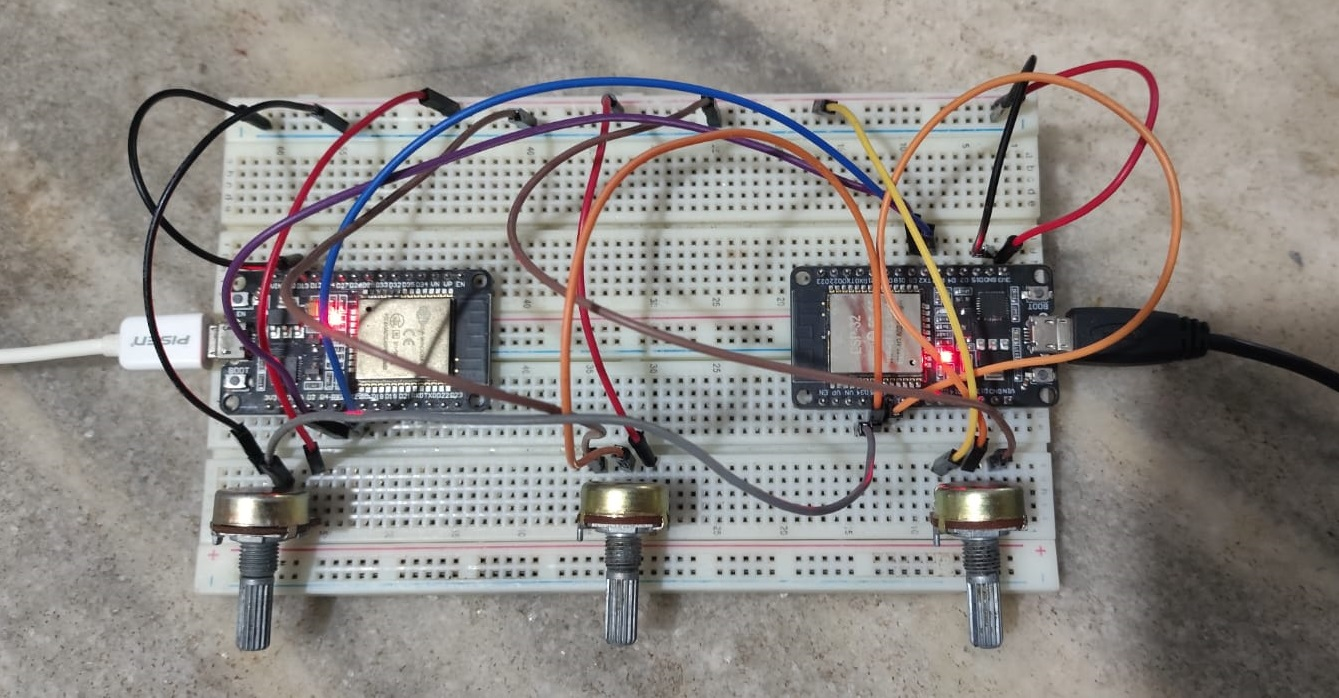
\includegraphics[width=.88\textwidth]{montagem_esp32.jpg}
\caption{Montagem experimental da plataforma, com os dois módulos ESP32, a protoboard e os três potenciômetros utilizados para modificar os parâmetros da planta.}
\label{fig:montagem_esp32}
\end{figure}

\begin{figure}[htbp]
\centering
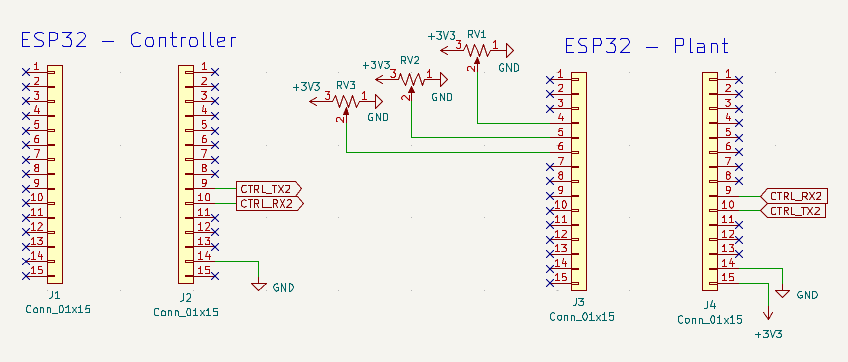
\includegraphics[width=.94\textwidth]{esquematico_esp32.png}
\caption{Esquemático das conexões da plataforma, incluindo a comunicação serial entre os ESP32 e as entradas analógicas associadas aos potenciômetros.}
\label{fig:esquematico_esp32}
\end{figure}

\subsubsection{Comunicação UART}

A comunicação entre controlador e planta foi implementada por UART, configurada com um baud rate de $115200 \mathrm{bit/s}$, $8$ bits de dados, sem bit paridade e um bit de parada. Para facilitar a sincronização entre dispositivos, foi definido um protocolo binário próprio, onde cada pacote possui um tamanho fixo de $15$ bytes. Como ilustrado na Figura~\ref{fig:pacotes_uart}, em cada pacote estão armazenados um cabeçalho de $2$ bytes, um contador de $8$ bytes, um campo de dados de $4$ bytes e um XOR Checksum de $1$ byte.

O cabeçalho, \texttt{0xFF66} para o controlador e \texttt{0xAA55} para a planta, serve para identificar o microcontrolador de origem e para delimitar o começo de um novo pacote. O contador auxilia na identificação de mensagens já processadas, descartando mensagems repetidas, enquanto o \textit{checksum} permite verificar a integridade do conteúdo recebido. As estruturas foram definidas como compactadas (\texttt{\_attribute\_((packed))}) de modo a evitar problemas devido aos bytes de \textit{padding} entre os campos.

\begin{figure}[htbp]
\centering
\begin{tikzpicture}[
 font=\small,
 packet/.style={draw=navyblue,line width=.7pt,minimum height=1.15cm,align=center,inner sep=2pt},
 note/.style={font=\scriptsize,align=center,text=black!65}
]
    \node[anchor=west,font=\bfseries] at (0,2.25) {Controlador $\rightarrow$ Planta};
    \node[packet,fill=lightblue,minimum width=2.1cm,anchor=west] (h1) at (0,1.2) {Cabeçalho\\\texttt{0xFF66}};
    \node[packet,minimum width=3.0cm,anchor=west] (c1) at (h1.east) {Contador\\\texttt{uint64\_t}};
    \node[packet,fill=warmgray,minimum width=2.45cm,anchor=west] (p1) at (c1.east) {Controle $u(k)$\\\texttt{float}};
    \node[packet,minimum width=2.0cm,anchor=west] (x1) at (p1.east) {Checksum\\XOR};
    \node[note,below=2mm of h1] {2 bytes};
    \node[note,below=2mm of c1] {8 bytes};
    \node[note,below=2mm of p1] {4 bytes};
    \node[note,below=2mm of x1] {1 byte};
    \node[anchor=west,font=\bfseries] at (0,-.35) {Planta $\rightarrow$ Controlador};
    \node[packet,fill=lightblue,minimum width=2.1cm,anchor=west] (h2) at (0,-1.4) {Cabeçalho\\\texttt{0xAA55}};
    \node[packet,minimum width=3.0cm,anchor=west] (c2) at (h2.east) {Contador\\\texttt{uint64\_t}};
    \node[packet,fill=warmgray,minimum width=2.45cm,anchor=west] (p2) at (c2.east) {Saída $y(k)$\\\texttt{float}};
    \node[packet,minimum width=2.0cm,anchor=west] (x2) at (p2.east) {Checksum\\XOR};
    \node[note,below=2mm of h2] {2 bytes};
    \node[note,below=2mm of c2] {8 bytes};
    \node[note,below=2mm of p2] {4 bytes};
    \node[note,below=2mm of x2] {1 byte};
\end{tikzpicture}
\caption{Estrutura dos pacotes UART. Definidos em utils.h.}
\label{fig:pacotes_uart}
\end{figure}

Duas tasks FreeRTOS, presentes em cada módulo, recebem e processam os pacotes: \texttt{uart\_rx\_task()} e \texttt{uart\_process\_task()}. A task de RX aguarda o recebimento de uma interrupção, setada pelo driver de UART, transfere os bytes recebidos para um buffer de análise e procura o cabeçalho do pacote. Uma vez identificado, verifica o \textit{checksum} e caso a mensagem for válida, encaminha-a para a task de processamento. Por sua vez, a task de processamento recebe a mensagem, verifica se é uma mensagem repetida, e dependendo do módulo faz tarefas diferentes. No controlador, a task armazena localmente a saída da planta; na planta, a task atualiza o estado interno do modelo.

\subsubsection{Organização do firmware}

O firmware foi estruturado em módulos separados para o controlador, a planta e o driver ADC. Para facilitar seu desenvolvimento todos os módulos compartilham o mesmo ambiente de trabalho, e por meio de uma opção de configuração do ESP-IDF, o usuario seleciona se o binário a ser compilado é da planta ou do controlador.

Devido à plataforma embarcada ter sido desenvolvida na framework ESP-IDF, a aplicação utiliza FreeRTOS de forma nativa, pelo qual foram usar tasks e callbacks de temporização FreeRTOS para o execução de diversas tarefas no código. Por conta de se tratar de uma aplicação com diversos contextos de execução, \textit{qeues} e \textit{mutexes} são empregados para transferir mensagens entre tasks e proteger variáveis compartilhadas.

Na Tabela~\ref{tab:tarefas_embarcadas} podem ser visualizadas as principais tasks e callback desenvolvidas. Todas as frequências informadas podem ser modificadas através da interfacede configuração do ESP-IDF, o \textit{menuconfig}.

\begin{table}[H]
    \centering
    \caption{Rotinas implementadas para os módulos do controlador e planta, e para o driver ADC.}
    \label{tab:tarefas_embarcadas}
    \fontsize{7.8}{9.6}\selectfont
    \renewcommand{\arraystretch}{1.22}
    \begin{tabularx}{\textwidth}{@{}p{1.6cm}p{4.0cm}p{2.35cm}X@{}}
        \toprule
        \textbf{Módulo} & \textbf{Callback associada} & \textbf{Acionamento} & \textbf{Função} \\
        \midrule
        Controlador & \texttt{controller\_timer\_callback()} & Temporizador periódico & Itera a malha de controle, atualizando o PI e enviando $u(k)$. \\
        Controlador & \texttt{uart\_rx\_task()} & Interrupção do UART & Recebe os dados da FIFO de RX do UART, encaminha pacotes validos para \texttt{uart\_process\_task()}. \\
        Controlador & \texttt{uart\_process\_task()} & Dado novo na queue FreeRTOS & Processa o pacote recebido, atualizando a variavel $y$ interna. \\
        Controlador & \texttt{mqtt\_timer\_callback()} & Temporizador periódico (20Hz) & Publica nos tópicos \texttt{ctrl/state} e \texttt{ctrl/ref}. \\
        Controlador & \texttt{mqtt\_event\_handler()} & Novo evento do cliente MQTT & Depuração da comunicação MQTT e recepção de dados do tópico \texttt{input/ref}. \\
        \midrule
        Planta & \texttt{uart\_rx\_task()} & Interrupção do UART & Recebe os dados da FIFO de RX do UART, encaminha pacotes validos para \texttt{uart\_process\_task()}. \\
        Planta & \texttt{uart\_process\_task()} & Dado novo na queue FreeRTOS & Processa o pacote recebido, atualiza o modelo farmacocinético e envia $y(k)$. \\
        Planta & \texttt{plant\_internals\_callback()} & Temporizador periódico (10Hz) & Lê o estado dos canais ADC e atualiza os parâmetros $\gamma_{ob}$, $\mu_m$ e $\mu_o$. \\
        Planta & \texttt{mqtt\_timer\_callback()} & Temporizador periódico (20Hz) & Publicação nos tópicos \texttt{plant/state} e \texttt{plant/internals}. \\
        Planta & \texttt{mqtt\_event\_handler()} & Novo evento do cliente MQTT & Depuração da comunicação MQTT. \\
        \midrule
        Driver ADC & \texttt{conv\_done\_cb()} & Interrupção do ADC & Notifica a tarefa de aquisição quando há suficientes amostras disponíveis no buffer do ADC. \\
        Driver ADC & \texttt{adc\_read\_task()} & Notificação de task FreeRTOS & Lê e processa as amostras do ADC1 em modo contínuo. \\
        \bottomrule
    \end{tabularx}
\end{table}

\subsubsection{Principio de funcionamento}

Um temporizador periódico, configurado em $100\mathrm{Hz}$ nominalmente, aciona a callback de processamento do controlador: \texttt{controller\_timer\_callback()}. A cada \textit{tick}, o controlador atualiza o controlador PI e gera a nova ação de controle $u(k)$. Dado que é fisicamente impossível administrar uma concentração negativa de remédio, a ação de controle é limitada inferiormente a zero. Diferente do controlador, a planta atualiza seu estado interno através da task \texttt{uart\_process\_task()}, a cada recebimento de um novo pacote valido do controlador. Assim, a frequência de atualização da planta depende da taxa de atualização do controlador. Para os testes com diferentes frequências foi suficiente modificar a frequência do controlador.

Por meio da rede Wi-Fi disponibilizada pela laptop os microcontroladores conseguem se conectar no broker Mosquitto, que permite a comunicação dos controladores com a dashboard por meio do protocolo MQTT. Internamente, a recepção de dados é controlada pela callback \texttt{mqtt\_event\_handler()}, enquanto a publicação é acionada por um temporizador periodico, que alerta \texttt{mqtt\_timer\_callback()}. Em uso, o ESP32 controlador recebe a referência no tópico \texttt{input/ref} e publica os dados de controle no tópico \texttt{ctrl/state}. Por sua vez, o ESP32 planta publica seus estados e saída em \texttt{plant/state}, além dos parâmetros internos variáveis em \texttt{plant/internals}. A publicação periódica dos dados ocorre nominal a $20\,\mathrm{Hz}$ em ambos os modulos.

A dashboard foi desenvolvida através das ferramentas Node-RED e FlowFuse. O fluxo da aplicação, ilustrado na Figura~\ref{fig:fluxo_nodered}, implementa nós de interface com o protocolo MQTT, os quais são processados pelos nós de "função" para compor a interface gráfica, cujos registros de operação são analisados na Subseção~\ref{subsec:resultados_embarcados}. 

\begin{figure}[htbp]
\centering
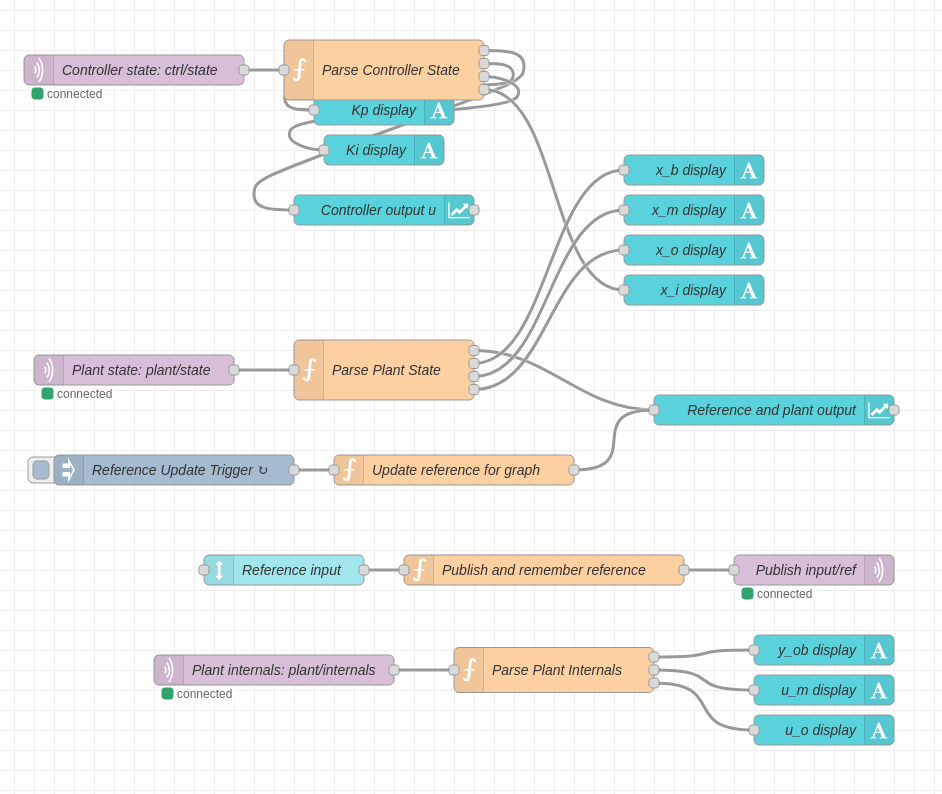
\includegraphics[width=.92\textwidth]{fluxo_nodered.jpg}
\caption{Fluxo de Node-RED}
\label{fig:fluxo_nodered}
\end{figure}

Visando testar a robustez da malha de controle projetada, os parâmetros variáveis do modelo farmacocinético podem ser modificados através do perirferico de ADC do ESP32 planta. Foram utilizados três potenciômetros alimentados em $3\mathrm{V}3$, conectados às entradas do periférico ADC1 do ESP32 planta. Os canais \texttt{ADC1\_CH4}, \texttt{ADC1\_CH6} e \texttt{ADC1\_CH7} são associados, respectivamente, aos parâmetros $\gamma_{ob}$, $\mu_m$ e $\mu_o$. Optou-se pelo ADC1 em razão da utilização simultânea do Wi-Fi, dado que no ESP32 o ADC2 é utilizado pelo API do sistema de comunicação sem fio.

O driver foi implementado utilizando o modo contínuo do ADC. Quando o buffer de conversão fica preenchido, o ADC gera uma interrupção e executa callback \texttt{conv\_done\_cb()}, notificando a task \texttt{adc\_read\_task()}. Essa task processa as amostras e calcula valores médios para cada canal. Em um contexto independete, numa frequência de $10 \mathrm{Hz}$ a callback \texttt{plant\_internals\_callback()} é acionada. Essa callback utiliza as leituras mais recentes do ADC ($a_4$,$a_6$ e $a_7$) para atualizar os parâmetros por meio das equações \eqref{eq:conversao_adc_parametros}, que associam os bits do ADC ($0 - 4095$) aos intervalos especificados no modelo: $\gamma_{ob}\in[0,037;0,040]$, $\mu_m\in[0,10;0,20]$ e $\mu_o\in[0,10;0,15]$.

\begin{equation}
    \begin{aligned}
        \gamma_{ob} &= 0,037 + \frac{0,003}{4095}\,a_4,\\
        \mu_m &= 0,1 + \frac{0,1}{4095}\,a_6,\\
        \mu_o &= 0,1 + \frac{0,05}{4095}\,a_7,
    \end{aligned}
    \label{eq:conversao_adc_parametros}
\end{equation}

\newpage
